\section{提案ツールの特長}

\begin{frame}{現状のイメージ開発の問題点}
    \vskip1.5zh
    開発時と動作確認時で,作業対象が異なる.
    \vskip1.5zh

    \begin{figure}
        \centering
        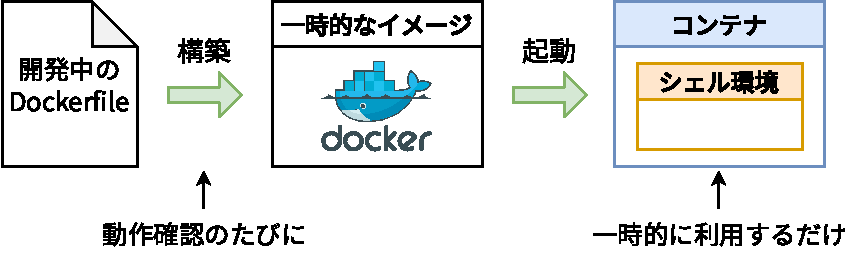
\includegraphics[width=\linewidth]{img/method1.pdf}
    \end{figure}

    \begin{onlyenv}<2>
        \begin{tikzpicture}[remember picture]
            \useasboundingbox (0.0, 0.0);
            \begin{scope}[shift={(current page.south west)}]
                \node[probrem] at (6.4, 4.6) {2つの問題が発生};
            \end{scope}
        \end{tikzpicture}
    \end{onlyenv}
\end{frame}


\begin{frame}{問題 1/2\\「Dockerfileの動作確認のオーバヘッド」}
    \vskip1.0zh
    Dockerfileを修正する度に,何度もイメージを構築する.

    → \textcolor{orange}{待ち時間が発生する}
    \vskip0.5zh

    \begin{figure}
        \centering
        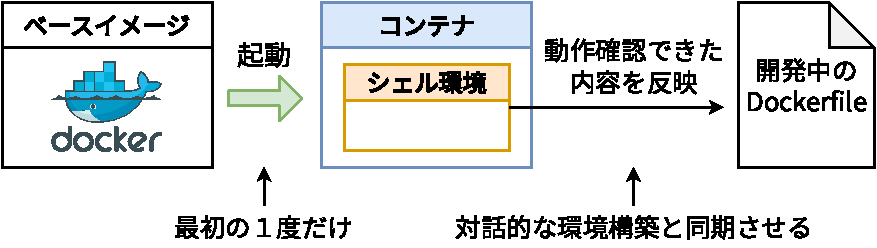
\includegraphics[width=\linewidth]{img/method2.pdf}
    \end{figure}
\end{frame}


\begin{frame}{問題 2/2\\「Dockerfile開発時の開発者の負担」}
    \vskip1.0zh
    目的の環境構築とDockerfileの編集作業を同時進行させる.

    → \textcolor{orange}{開発者の負担が大きい}
    \vskip0.5zh

    \begin{figure}
        \centering
        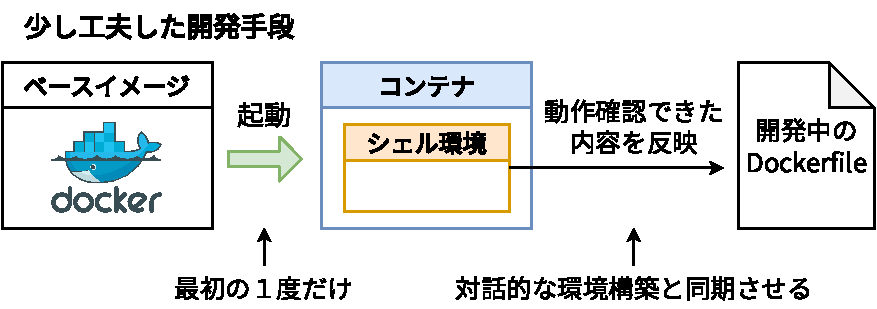
\includegraphics[width=\linewidth]{img/method3.pdf}
    \end{figure}
\end{frame}


\begin{frame}{提案ツールを用いて,Dockerfileを開発すると}
    \begin{figure}
        \centering
        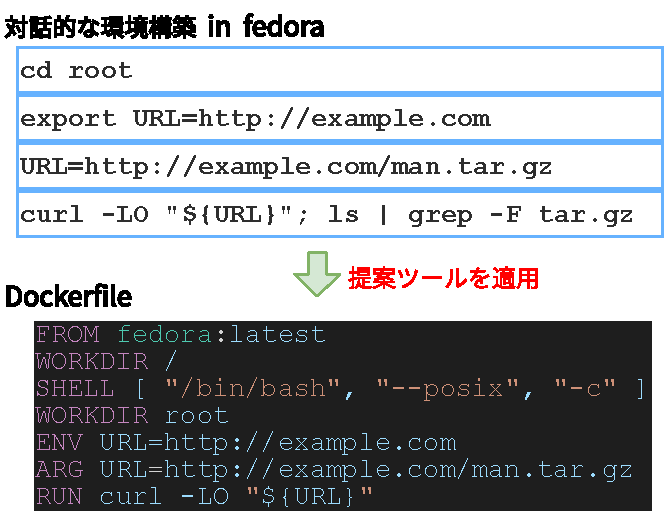
\includegraphics[width=0.95\linewidth]{img/outline.pdf}
    \end{figure}
\end{frame}


\begin{frame}{提案ツールの特長 1/2}
    \textcolor{blue!75}{\large インタラクティブツールとしての側面}

    ユーザがコンテナ内で動作確認しながら環境構築することで,自動的にDockerfileを生成してくれる.
\end{frame}


\begin{frame}{これだけでは優れたDockerfileにはならない}
    \begin{figure}
        \centering
        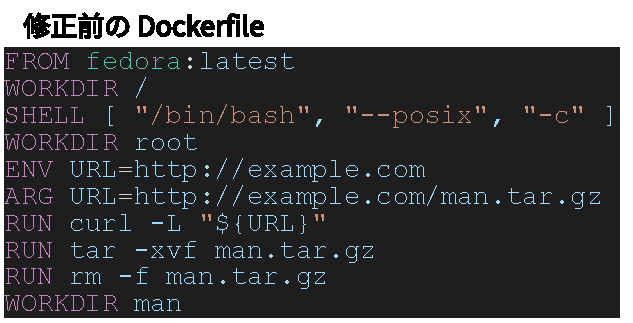
\includegraphics[width=1.02\linewidth]{img/optimize1.pdf}
    \end{figure}

    \begin{tikzpicture}[remember picture]
        \useasboundingbox (0.0, 0.0);
        \begin{scope}[shift={(current page.south west)}]
            \only<2>{\node[probrem] at (6.4, 4.0) {見づらい};}

            \begin{onlyenv}<3>
                \node[callout, callout absolute pointer={(5.6, 4.8)}] at (8.6, 6.6) {絶対パス指定の方がいい};
                \node[callout, callout absolute pointer={(6.4, 3.4)}] at (9.0, 2.0) {集約した方がいい};
                \node[callout, callout absolute pointer={(7.2, 4.2)}] at (9.0, 2.0) {集約した方がいい};
            \end{onlyenv}
        \end{scope}
    \end{tikzpicture}
\end{frame}


\begin{frame}{Dockerfileのリファクタリング・最適化を行ってみる}
    \begin{figure}
        \centering
        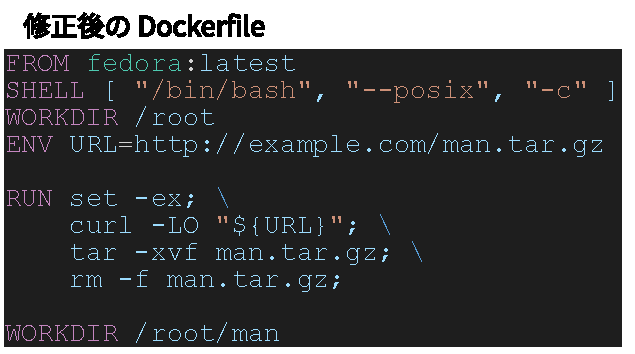
\includegraphics[width=1.02\linewidth]{img/optimize2.pdf}
    \end{figure}
\end{frame}


\begin{frame}{提案ツールの特長 2/2}
    \textcolor{blue!75}{\large インタラクティブツールとしての側面}

    ユーザがコンテナ内で動作確認しながら環境構築することで,自動的にDockerfileを生成してくれる.

    \vskip2.0zh
    \textcolor{blue!75}{\large リファクタリング・最適化の機能}

    上のようにして生成したDockerfileに,ベストプラクティスに基づいたリファクタリング・最適化を行うことができる.
\end{frame}